\section{Auswertung}
\subsection{Isobare Molwärme}
Um die Molwärme bei konstantem Druck aus den gegebenen Messwerten zu bestimmen, muss zunächst die Zeitdifferenz für alle gemessenen Zeiten errechnet werden. Aus dieser kann dann die elektrische Energie mit der Formel \eqref{eenergie} berechnet werden. Die Temperatur aus dem Widerstand mit Hilfe der Formel \eqref{pt100} bestimmt.

\noindent Mit diesen Werten kann nun die spezifische Wärme berechnet werden. Die Molwärme ergibt sich dann aus Formel \eqref{cp_mol}.

\noindent Die benutzten Messwerte sind Tabelle \ref{fig:tab1} zu entnehmen.   

\begin{table}[H]
	\begin{center}
		\begin{tabular}{c c c c c c}
			\toprule
			\(t\)/s & \(R\)/\(\Omega\) & \(I\)/mA & \(U\)/V & \(T\)/K & \(\sigma_T\)/K\\
			\midrule
			0		&22,2		&133,9	&14,14	&81,76	&0,24 \\
			300		&25,2		&136,0	&14,24	&88,84	&0,24 \\
			600		&27,6		&146,1	&15,32	&94,52	&0,24 \\
			900		&30,0		&160,0	&16,79	&100,22	&0,24 \\
			1200	&33,1		&166,4	&17,48	&107,60	&0,24 \\
			1500	&36,2		&175,7	&18,49	&115,00	&0,24 \\
			1800	&39,2		&180,3	&18,98	&122,19	&0,24 \\
			2100	&44,9		&180,8	&18,98	&135,92	&0,24 \\
			2400	&48,8		&180,0	&18,98	&145,37	&0,24 \\
			2700	&52,7		&180,3	&18,98	&154,85	&0,24 \\
			3000	&56,3		&180,4	&18,98	&163,64	&0,24 \\
			3300	&59,8		&180,5	&18,98	&172,22	&0,25 \\
			3600	&63,3		&180,6	&18,98	&180,84	&0,25 \\
			3900	&66,6		&180,7	&18,98	&188,99	&0,25 \\
			4260	&70,4		&180,8	&18,98	&198,41	&0,25 \\
			4620	&73,3		&180,9	&18,98	&205,63	&0,25 \\
			4980	&77,8		&181,0	&18,98	&216,87	&0,25 \\
			5340	&81,0		&181,0	&18,98	&224,89	&0,25 \\
			5760	&85,6		&181,1	&18,98	&236,48	&0,25 \\
			6120	&89,0		&181,1	&18,98	&245,09	&0,25 \\
			6480	&92,5		&181,2	&18,98	&253,98	&0,25 \\
			6840	&96,1		&181,2	&18,98	&263,15	&0,26 \\
			7200	&99,7		&181,3	&18,98	&272,36	&0,26 \\
			7560	&102,5		&181,3	&18,98	&279,55	&0,26 \\
			7980	&106,6		&181,3	&18,98	&290,11	&0,26 \\
			8400	&110,2		&181,3	&18,98	&299,42	&0,26 \\
			\bottomrule
		\end{tabular}
		\caption{Messdaten und Temperatur}
		\label{fig:tab1}
	\end{center}
\end{table}

\noindent Hierbei wird für die Zeit ein Reaktionsfehler von \(\sigma_t=1\text{s}\), für den Widerstand ein Ablesefehler von \(\sigma_\Omega=0,1\text{Ohm}\) und für Strom und Spannung jeweils ein Ablesefehler von \(\sigma_I=0,01\text{mA}\) und \(\sigma_U=0,01\text{V}\) angenommen.

\noindent Da in der Molwärme und Energie Differenzen auftreten, wird der letzte Messwert nicht mehr in die Berechnung eingehen.

\noindent Die Messunsicherheit der Energie berechnet sich aus der Formel für die Gauß'sche Fehlerfortpflanzung:
\begin{equation}
\sigma_E=\sqrt{(I\Delta t\cdot\sigma_U)^2 + (U\Delta t\cdot\sigma_I)^2 + (UI\cdot\sigma_t)^2}
\end{equation}

\noindent Die Messunsicherheit für die Molwärme errechnet sich zu:
\begin{equation}
\sigma_{C_p}=\sqrt{\left(\frac mM\cdot\frac{1}{\Delta t}\cdot\sigma_E\right)^2+\left(-\frac mM\cdot\frac{E}{\Delta t^2}\cdot\sigma_t\right)^2 }
\end{equation}

\noindent Die Ergebnisse für die Molwärme und Energie sind Tabelle \ref{fig:tab2} zu entnehmen.

\begin{table}[H]
	\begin{center}
		\begin{tabular}{c c c c c c}
			\toprule
			\(E\)/J & \(\sigma_E\)/J & \(\Delta t\)/s & \(\Delta T\)/K & \(C_p\)/\(\frac{\text{J mol}}{\text{K}}\) & \(\sigma_{C_p}\)/							\(\frac{\text{J mol}}{\text{K}}\) \\
			\midrule
			568,00	&2,68	&300	&81,76	&14,91	&0,71\\
			580,99	&2,74	&300	&88,84	&19,00	&1,12\\
			671,48	&3,17	&300	&94,52	&21,91	&1,30\\
			805,92	&3,79	&300	&100,22	&20,29	&0,93\\
			872,60	&4,11	&300	&107,59	&21,89	&1,00\\
			974,61	&4,59	&300	&115,00	&25,18	&1,19\\
			1026,62	&4,84	&300	&122,19	&13,89	&0,35\\
			1029,48	&4,85	&300	&135,92	&20,26	&0,74\\                           
			1024,92	&4,83	&300	&145,37	&20,08	&0,86\\
			1026,63	&4,84	&300	&154,85	&21,69	&0,86\\ 
			1027,20	&4,84	&300	&163,64	&22,24	&0,90\\
			1027,76	&4.85	&300	&172,22	&22,17	&0,90\\
			1028,34	&4,85	&300	&180,84	&23,44	&1,01\\
			1234,69	&4,85	&360	&188,99	&24,35	&0,91\\
			1235,37	&4,85	&360	&198,41	&31,81	&1,56\\
			1236,05	&4.86	&360	&205,63	&20,43	&0,65\\
			1236,74	&4.86	&360	&216,87	&28,63	&1,27\\                
			1442,86	&4.86	&360	&224,89	&23,14	&0,76\\                  
			1237,42	&4.86	&360	&236,40	&26,73	&1,12\\                    
			1237,42	&4.86	&360	&245,09	&25,87	&1,05\\
			1238,10	&4.86	&360	&253,98	&25,07	&0,98\\ 
			1238,10	&4.86	&360	&263,15	&24,97	&0,99\\            
			1238,78	&4.86	&360	&272,36	&32,02	&1,62\\
			1445,25	&4.86	&420	&279,55	&25,43	&0,88\\
			1445,25	&4.86	&420	&290,11	&28,84	&1,14\\
			\bottomrule
		\end{tabular}
		\caption{Werte für die zugeführte Energie und die davon errechnete Molwärme}
		\label{fig:tab2}
	\end{center}
\end{table}

\subsection{Isochore Molwärme}
Die Molwärme bei konstantem Volumen wird über die Korrekturformel \eqref{kf} berechnet. Hierzu ist das Wissen über die Werte des Ausdehnungskoeffizienten von Relevanz. In Abbildung \ref{fig:tab3} sind Werte für \(\alpha\) für bestimmte Temperaturen angegeben.

\begin{table}[H]
	\begin{center}
		\begin{tabular}{c c}
			\toprule
			\(T\)/K & \(\alpha/\text{K}\cdot10^{-6}\)\\
			\midrule
			70	&7,00\\
			80	&8,50\\
			90	&9,75\\
			100	&10,70\\
			110	&11,50\\
			120	&12,10\\
			130	&12,65\\
			140	&13,15\\
			150	&13,60\\
			160	&13,90\\
			170	&14,25\\
			180	&14,50\\
			190	&14,75\\
			200	&14,95\\
			210	&15,20\\
			220	&15,40\\
			230	&15,60\\
			240	&15,75\\
			250	&15,90\\
			260	&16,10\\
			270	&16,25\\
			280	&16,35\\
			290	&16,50\\
			300	&16,65\\
			\bottomrule
		\end{tabular}
		\caption{Linearer Ausdehnungskoeffizient \(\alpha\) von Kupfer in Abhängigkeit von der Temperatur}
		\label{fig:tab3}
	\end{center}
\end{table}

\noindent Um Werte für die gegebenen Temperaturen aus Tabelle \ref{fig:tab1} zu bekommen, werden die Werte aus Tabelle \ref{fig:tab3} als Stützstellen mit Hilfe eines Polynoms sechsten Grades interpoliert:

\begin{equation*}
p(x)=ax^6+bx^5+cx^4+dx^3+ex^2+fx+g\quad.
\end{equation*}

\begin{figure}
	\centering
		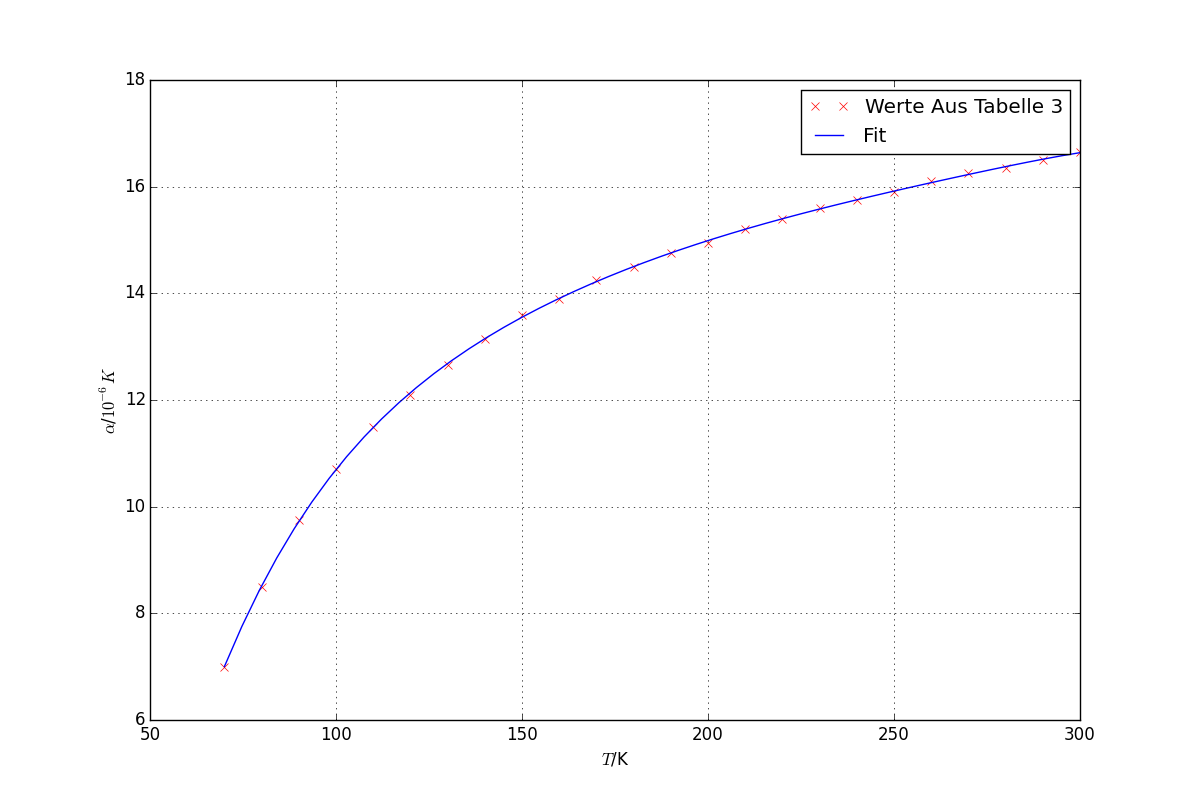
\includegraphics[width=0.5\textwidth]{inter.png}
	\caption{Interpolation des Polynoms}
	\label{fig:abb1}
\end{figure}

\noindent Für die Korrekturformel wird noch der Kompressionsmodul und das Molvolumen benötigt. Hierfür werden Literaturwerten verwendet: \(\kappa=1,378\cdot10^{11}\frac{\text{N}}{\text{m}^2}\), \(V_0=7,11\cdot10^{-6}\frac{\text{m}^3}{\text{mol}}\). 

\noindent Die Werte für die Molwärme und die passenden Ausdehnungskoeffizienten sind der Tabelle \ref{fig:tab4} zu entnehmen.

\begin{table}[H]
	\begin{center}
		\begin{tabular}{c c c c c}
			\toprule
			\(T\)/K & \(\alpha/\text{K}\cdot10^{-6}\) & \(\sigma_\alpha/\text{K}\cdot10^{-5}\) & \(C_V\)/\(\frac{\text{J mol}}{\text{K}}\) & \(\sigma_{C_V}\)\(\frac{\text{J mol}}{\text{K}}\) \\
			\midrule
			81,76&	8,75		&1,38	&14,85	&0,72\\
			88,84&	9,59		&1,63	&18,93	&1,14\\
			94,52&	10,18	&1,85	&21,82	&1,33\\
			100,22&	10,71	&2,11	&20,19	&1,01\\
			107,60&	13,10	&2,48	&21,77	&1,13\\
			115,00&	11,82	&2,90	&25,04	&1,38\\
			122,19&	12,27	&3,37	&13,73	&0,95\\
			135,92&	12,97	&4,44	&20,05	&1,56\\
			145,37&	13,37	&5,34	&19,85	&1,97\\
			154,85&	13,73	&6,38	&21,44	&2,54\\
			163,64&	14,02	&7,49	&21,96	&3,16\\
			172,22&	14,29	&8,73	&21,86	&3,89\\
			180,84&	14,52	&10,15	&23,10	&4,80\\
			188,99&	14,73	&11,65	&23,98	&5,79\\
			198,41&	14,95	&13,63	&31,41	&7,30\\
			205,63&	15,11	&15,32	&20,01	&8,42\\
			216,87&	15,34	&18,32	&28,17	&10,82\\
			224,89&	15,49	&20,74	&22,66	&12,76\\
			236,48&	15,69	&24,71	&26,21	&16,21\\
			245,09&	15,84	&28,04	&25,33	&19,22\\
			253,98&	15,98	&31,89	&24,50	&22,84\\
			263,15&	16,12	&36,30	&24,37	&27,18\\
			272,36&	16,26	&41,23	&31,39	&32,25\\
			279,55&	16,37	&45,46	&24,76	&36,70\\
			290,11&	16,51	&52,33	&28,14	&44,23\\
			\bottomrule
		\end{tabular}
		\caption{Ausdehnungskoeffizient für gemessene Temperaturen und Molwärme bei konstantem Volumen}
		\label{fig:tab4}
	\end{center}
\end{table}

\noindent Die Messunsicherheit \(\sigma_\alpha\) ergibt sich aus:

\begin{equation}
\sigma_\alpha=\sqrt{((6aT^5+5bT^4+4cT^3+3ddT^2+2eT+f)\sigma_T)^2+(T^5\cdot\sigma_a)^2+(T^4\cdot\sigma_b)^2+(T^3\cdot\sigma_c)^2+(T^2\cdot\sigma_d)^2+(T\cdot\sigma_e)^2+(\sigma_f)^2+(0\cdot\sigma_g)^2}
\end{equation}

\noindent Die Messunsicherheit für die isochore Molwärme ergibt sich aus:

\begin{equation}
\sigma_{C_V}=\sqrt{(\Delta\sigma_{C_p})^2 + (9\alpha^2\kappa V_0\cdot\sigma_T)^2 + (18\alpha\kappa V_0T\cdot\sigma_\alpha)^2}
\end{equation}

\noindent Die Molwärme bei konstantem Volumen gegen die Temperatur im linearen Diagramm wird in Abbildung \ref{fig:abb2} dargestellt.

\begin{figure}
	\centering
		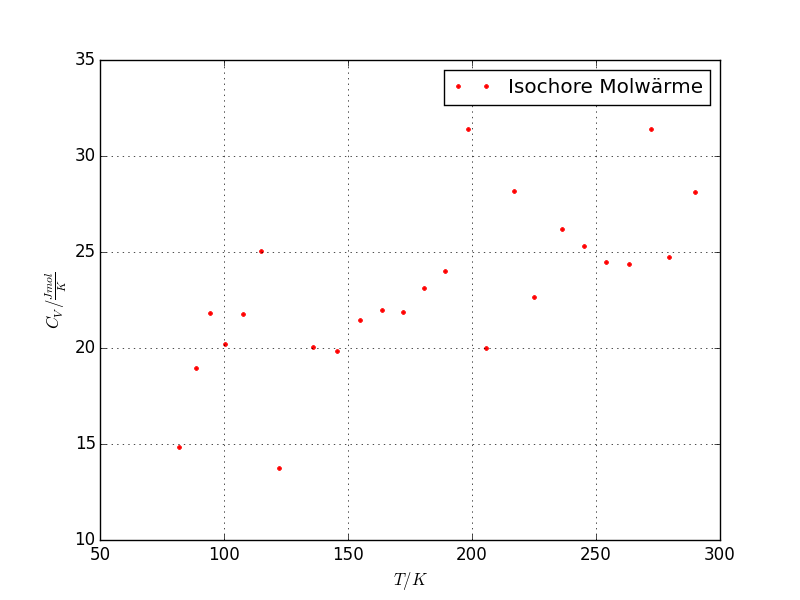
\includegraphics[width=0.5\textwidth]{cv.png}
	\caption{Isochore Molwärme und Grenzwert}
	\label{fig:abb2}
\end{figure}

\subsection{Debye-Temperatur}
Die Werte für\(\frac{\theta_\text{D}}{T}\) werden aus Tabelle \ref{fig:tab4} bestimmt. Dabei sind die Zahlen der ersten Spalte die Nachkommastellen. Die Debye-Temperatur wird dann durch Multiplikation mit der Temperatur berechnet. Das Ergebnis ist Tabelle \ref{fig:tab5} zu entnehmen.

\begin{figure}
	\centering
		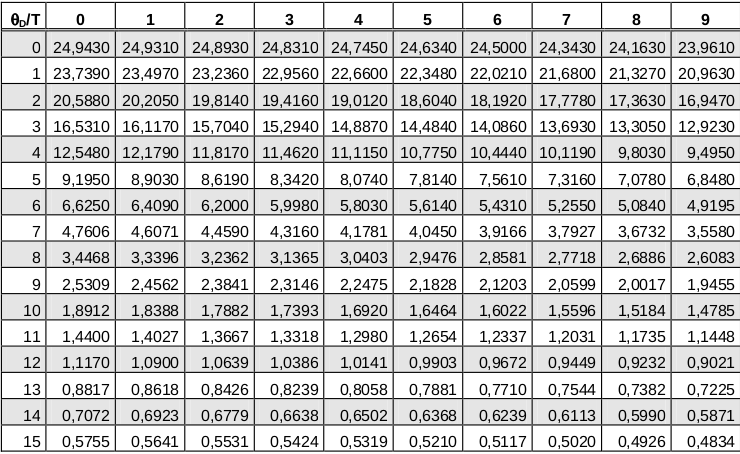
\includegraphics[width=0.5\textwidth]{debye.png}
	\caption{Debye-Temperatur für bestimmte Molwärme}
	\label{fig:abb3}
\end{figure}

\begin{table}[H]
	\begin{center}
		\begin{tabular}{c c c c}
			\toprule
			\(T\)/K & \(C_V\)/\(\frac{\text{J mol}}{\text{K}}\) & \(\frac{\theta_\text{D}}{T}\) & \(\theta_D\)/K \\
			\midrule
			81,76	&14,85	&4,3		&351,57\\
			88,84	&18,93	&4,2		&373,13\\
			94,52	&21,82	&7,1		&671,09\\
			100,22	&20,19	&1,2		&120,26\\
			107,60	&21,77	&7,1		&763,96\\
			115,00	&25,04	&0,0		&0,00\\
			122,19	&13,73	&7,3		&891,99\\
			135,93	&20,05	&2,2		&299,02\\
			145,37	&19,85	&2,2		&319,81\\
			154,85	&21,44	&8,1		&1254,29\\
			163,64	&21,96	&6,1		&998,20\\
			\bottomrule
		\end{tabular}
		\caption{Ergebnisse für die Debye-Temperatur}
		\label{fig:tab5}
	\end{center}
\end{table}

\noindent Der Wert \(C_V\) ist offensichtlich ein Messfehler, weswegen er nicht in die Berechnung des Mittelwerts eingeht.

\noindent Der Mittelwert dieser Werte für die Debye-Temperatur lautet dann:

\begin{equation}
\frac{1}{10}\sum\limits_{i=1}^{10}{\theta_{\text{D}}}_i=\overline{\theta_\text{D}}=549,39
\end{equation}

\noindent Die Standardabweichung ist dann:

\begin{equation}
\sigma_\theta=\sqrt{\frac{1}{9}\sum\limits_{i=1}^{10}({\theta_{\text{D}}}_i-\overline \theta_{\text{D}})^2}=118,63
\end{equation}

\subsection{Debye-Frequenz}
Zur Berechnung der theoretischen Debye-Frequenz wird die Forderung \eqref{debyeintegral} betrachtet. Aus dieser folgt der Ausdruck \eqref{debyefreq}, mit dem es möglich ist, die Debye-Frequenz analytisch zu bestimmen.

\noindent Die noch zu bestimmenden Größen sind die Teilchenzahl \(N_L\) und das Volumen der Probe \(L^3\).

\begin{equation*}
N_L=\frac{m}{m_\text{Atom}}=\frac{0,342\text{kg}}{63,55\cdot 1,66\cdot10^{-27}\text{kg}}=3,24\cdot10^{24}
\end{equation*}

\begin{equation*}
L^3=\frac{m}{\rho_\text{Kupfer}}=\frac{0,342\text{kg}}{8,92\cdot10^3\frac{kg}{\text{m}^3}}=3,83\cdot10^{-5}\text{m}^3
\end{equation*}

\noindent Dabei ist \(m_\text{Atom}\) die Masse eines einzelnen Kupferatoms. Für die Geschwindigkeiten wird \(v_\text{long}=4,7\cdot10^3\frac{\text{m}}{\text{s}}\) und \(v_\text{trans}=2,26\cdot10^3\frac{\text{m}}{\text{s}}\) verwendet.

\noindent Daraus ergibt sich für die Debye-Frequenz:

\begin{equation*}
\omega_\text{D}=5,38\cdot10^{13}\frac{1}{\text{s}}
\end{equation*}

\noindent Daraus lässt sich auch die theoretische Debye-Temperatur berechnen. Gemäß $\theta_\text{D}=\frac{\hbar\omega_\text{D}}{k}$ lautet die theoretische Temperatur:

\begin{equation*}
\theta_\text{D}=411,22\text{K}\quad.
\end{equation*}